\section{DynamoDB and QuickSight - Zhaoheng Wang}
	\subsection{Data structure organization}
    The general process of our project is to parse the file which contains sample data and load into database. After that, we will do the analysis base on the processed data. Before loading data into DynamoDB, the table and the data structure should be organized. Therefore, the first job for me is to figure out the data structure before creating table. DynamoDB is actually a key-value type NoSQL which is different from the Mysql (the key-value type relational database). In relational database, the ER-diagram is usually used to convert data into schema. In the key-value type of NoSQL database, the ER-diagram is not suitable to represent the table. So I have do some research about how to organizing data structure in DynamoDB. From the research, there are two ways I find to organizing data structure in DynamoDB. The first one is to convert from ER-diagrams however, it only gives general idea about this not specific step. Therefore, I choose the second way for organizing data structure. In this way, we treat each rows of sample data as an individual item and each columns will be the attributes for the item. When we load the data into table, we are actually load the items into the table in DynamoDB. For instance, we need to store the wireless information for different users based on sample data such as connecting time, disconnecting time, information of device, average usage and operating system they use. In this case, we treat each user as individual items and the wireless information for that user will be the attributes.
    \subsection{Table creation}
    After data structure have been organized, the next job for me is to creating table in DynamoDB. The tool we choose is AWS java SDK. AWS Java SDK is similar with the command line prompt in Windows. we could use it to do different implementations for the table such as creating table, do updating. For instance, if we need to update some items(not large quality) in the table, we could use the APIs in AWS Java SDK to create table. Because of the APIS offered by AWS java SDK document, this step will be much easier than before. However, AWS Java SDK is not efficient for uploading the items if there are very large quality of items. As a result, we will only use it for simple operations such as creating table, deleting table, updating table. We finish creating table and loading sample data on Wednesday of week 5.
\subsection{QuickSight}
	\subsubsection{QuickSight graph creation}
    After the table is created and the data has been load into DynamoDB. We step to make visualization on QuickSight at the end of week 5. We follow step on the Quicksight document for creating the visual. For our project, the first step is to generate a data source in s3 or local pc. These data source are very important for Quicksight because it will require these data source for creating data set and do the analyzing. After that, the Quicksight needs to connect with the data source. In this step, if the database is on the Amazon web services the data source will be easily to connect. However, if the data source is not on the Amazon web services it requires database access information to connect the data source in database. For our project, since the s3 is on AWS it is easy to connect with data source. The next step is to create the data set according to data source and do an analyzing. After the data set has been created, the visual can be generated by the data set. There are different types of visual on the Quicksight and we can choose one to generate the suitable graph for the analyzing results.
	\subsubsection{Improvement in future}
    Currently, we have finished data structure organizing, creating table and make visualization based on the sample data. However, there still have some improvement for these parts in our project. Firstly, the way I choose for design the data structure may not be the optimal choice. Therefore, I would like to check with the data analyzer whether it is the efficient way or not. Secondly, the graph which made by QuickSight needs to improve because some of sample data needs to be filter. Furthermore, the QuickSight seems not handle the complex analysis and our client doesn’t give specific topic that we need to analysis. As a result, I would like to check with the data analyzer what kind of analysis we need to do.
    \subsubsection{Screenshot of the image on QuickSight}
    The figure \ref{fig:1} shows Proportion of Different OS which users use to access.Based on the graph, most of users are using Mac OS or IOS to access the wireless.The figure \ref{fig:2} the relationship between different OS and total Traffic. As we can see, the ios system will be the highest one.The figure \ref{fig:3} the Relationship of Total Traffic in different connecting time and Avg Usage in different Connecting Time.The figure \ref{fig:4} shows the relationship Between Total Traffic, Avg Usage and Device Name
 \begin{figure}[H]
 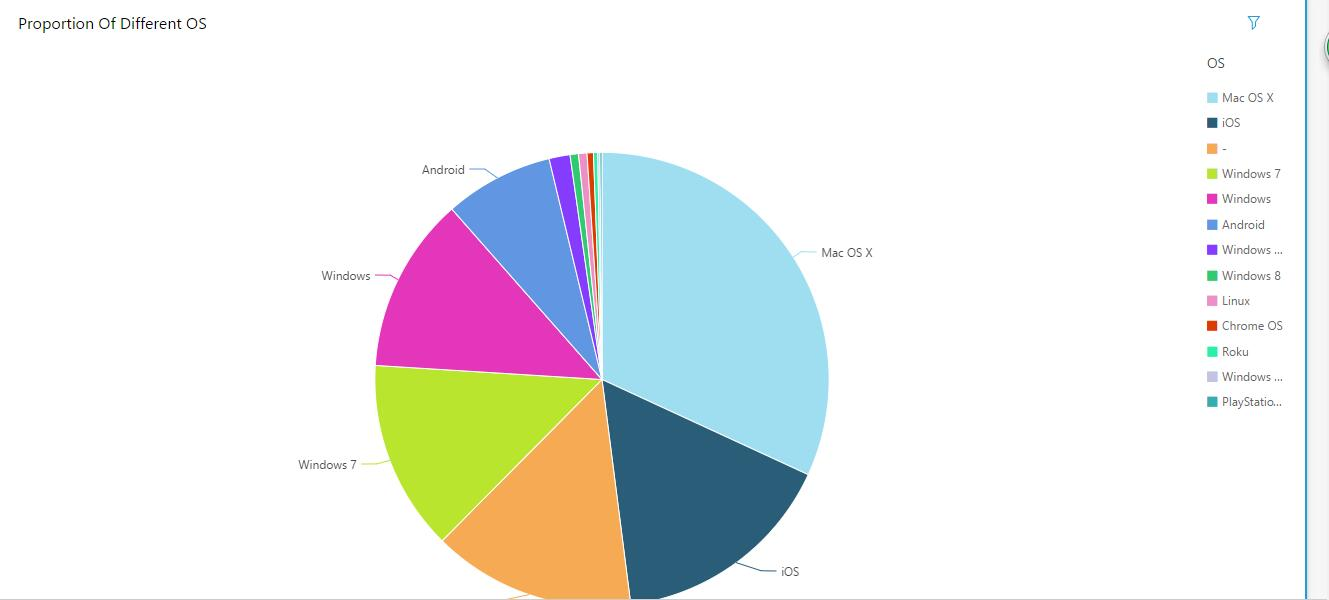
\includegraphics[width=17cm, height=8cm]{1.jpg}
 \centering
 \caption{\label{fig:1}Proportion of Different OS}
 \end{figure}
 
 \begin{figure}[H]
 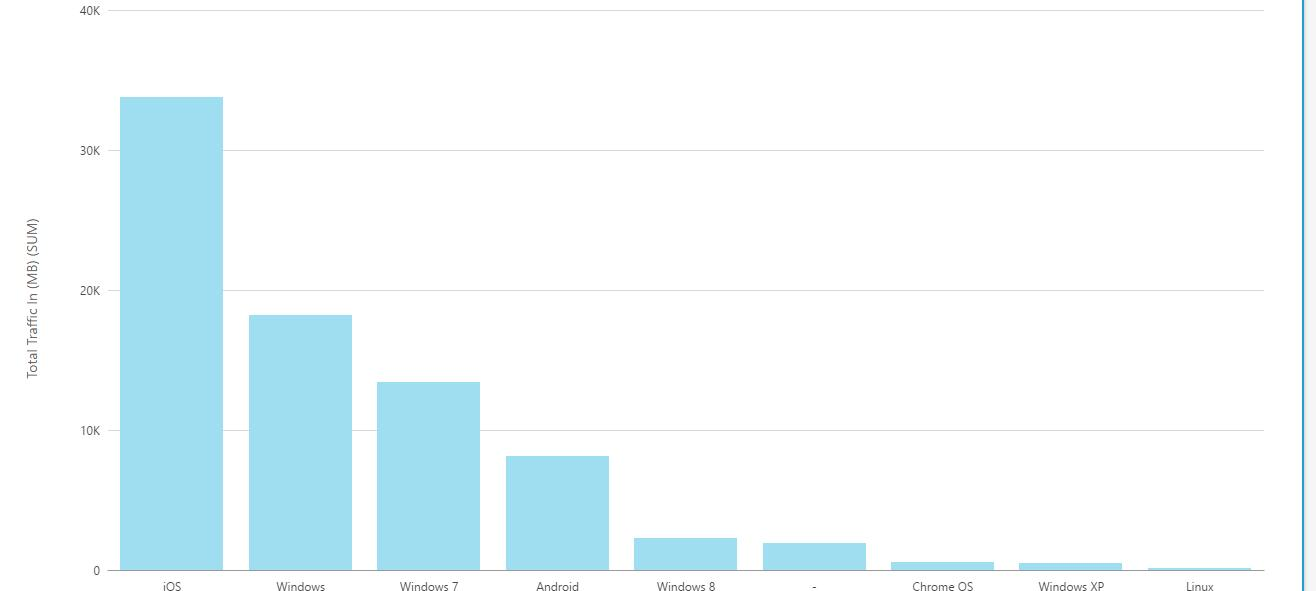
\includegraphics[width=17cm, height=8cm]{2.jpg}
 \centering
 \caption{\label{fig:2}relationship between different OS and total Traffic}
 \end{figure}

 \begin{figure}[H]
 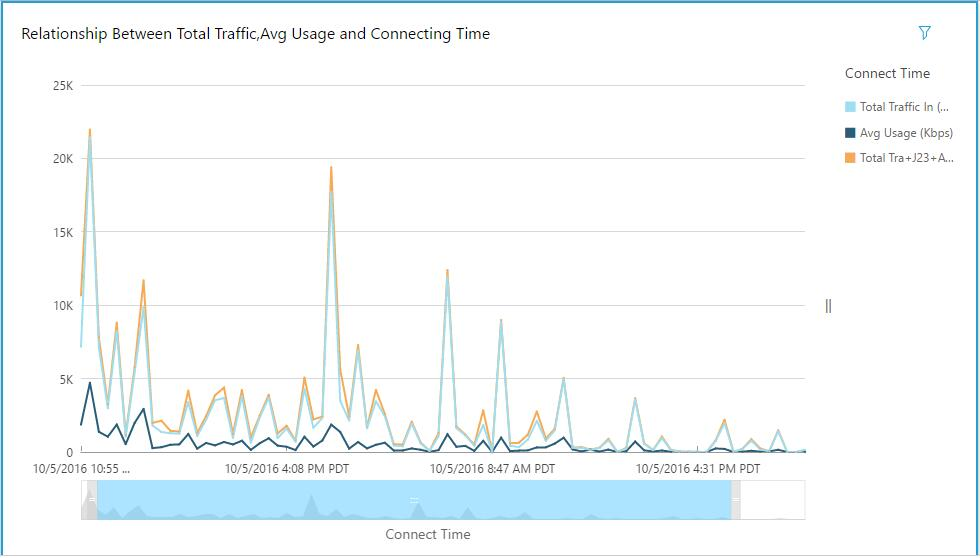
\includegraphics[width=17cm, height=8cm]{4.jpg}
 \centering
 \caption{\label{fig:3}relationship between different OS and total Traffic}
 \end{figure}
 
 \begin{figure}[H]
 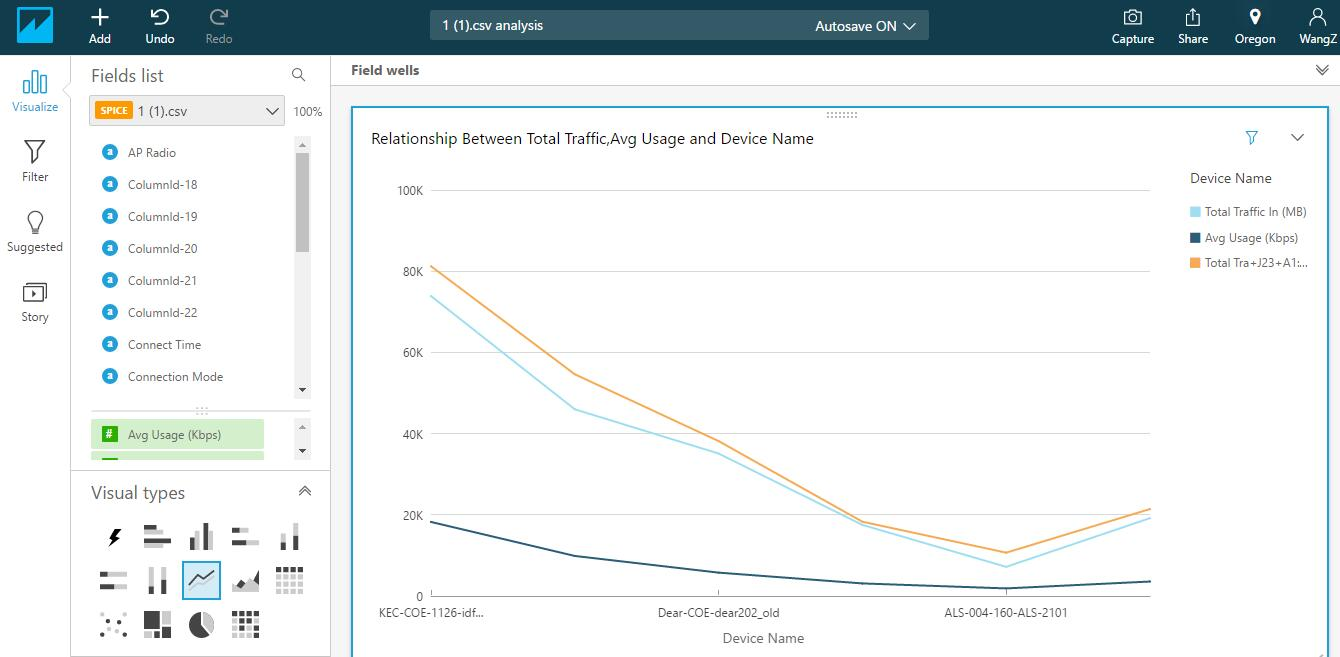
\includegraphics[width=17cm, height=8cm]{5.jpg}
 \centering
 \caption{\label{fig:4}relationship between different OS and total Traffic}
 \end{figure}

 
 
	